\documentclass[twoside]{article}
\setlength{\oddsidemargin}{0.25 in}
\setlength{\evensidemargin}{-0.25 in}
\setlength{\topmargin}{-0.6 in}
\setlength{\textwidth}{6.5 in}
\setlength{\textheight}{8.5 in}
\setlength{\headsep}{0.75 in}
\setlength{\parindent}{0 in}
\setlength{\parskip}{0.1 in}
\newcommand{\eqdef}{:\mathrel{\mathop=}}
\newcommand{\norm}[1]{\left\lVert #1 \right\rVert}

%
% ADD PACKAGES here:
%

\usepackage{amsmath,amsfonts,graphicx,dsfont,amssymb, cool, cancel}
%
% The following commands set up the lecnum (lecture number)
% counter and make various numbering schemes work relative
% to the lecture number.
%
\newcounter{lecnum}
\renewcommand{\thepage}{\thelecnum-\arabic{page}}
\renewcommand{\thesection}{\thelecnum.\arabic{section}}
\renewcommand{\theequation}{\thelecnum.\arabic{equation}}
\renewcommand{\thefigure}{\thelecnum.\arabic{figure}}
\renewcommand{\thetable}{\thelecnum.\arabic{table}}
\newcommand{\indep}{\raisebox{0.05em}{\rotatebox[origin=c]{90}{$\models$}}}

%
% The following macro is used to generate the header.
%
\newcommand{\lecture}[4]{
   \pagestyle{myheadings}
   \thispagestyle{plain}
   \newpage
   \setcounter{lecnum}{#1}
   \setcounter{page}{1}
   \noindent
   \begin{center}
   \framebox{
      \vbox{\vspace{2mm}
    \hbox to 6.28in { {\bf Advanced Machine Learning
	\hfill Fall 2020} }
       \vspace{4mm}
       \hbox to 6.28in { {\Large \hfill Lecture #1: #2  \hfill} }
       \vspace{2mm}
       \hbox to 6.28in { {\it  #3 \hfill  #4} }
      \vspace{2mm}}
   }
   \end{center}
   \markboth{Lecture #1: #2}{Lecture #1: #2}

   {\bf Note}: {\it LaTeX template courtesy of UC Berkeley EECS dept.}

   {\bf Disclaimer}: {\it These notes are adapted from ETH's Advanced Machine Learning Course, "Linear Regression via Maximization of the Likelihood, COS 234, Princeton", "The Elements of Statistical Learning, Chapter 3, Springer" and "Pattern Recognition and Machine Learning, Chapter 3, Springer".}
   \vspace*{4mm}
}
%
% Convention for citations is authors' initials followed by the year.
% For example, to cite a paper by Leighton and Maggs you would type
% \cite{LM89}, and to cite a paper by Strassen you would type \cite{S69}.
% (To avoid bibliography problems, for now we redefine the \cite command.)
% Also commands that create a suitable format for the reference list.
\renewcommand{\cite}[1]{[#1]}
\def\beginrefs{\begin{list}%
        {[\arabic{equation}]}{\usecounter{equation}
         \setlength{\leftmargin}{2.0truecm}\setlength{\labelsep}{0.4truecm}%
         \setlength{\labelwidth}{1.6truecm}}}
\def\endrefs{\end{list}}
\def\bibentry#1{\item[\hbox{[#1]}]}

%Use this command for a figure; it puts a figure in wherever you want it.
%usage: \fig{NUMBER}{SPACE-IN-INCHES}{CAPTION}
\newcommand{\fig}[3]{
			\vspace{#2}
			\begin{center}
			Figure \thelecnum.#1:~#3
			\end{center}
	}
% Use these for theorems, lemmas, proofs, etc.
\newtheorem{theorem}{Theorem}[lecnum]
\newtheorem{lemma}[theorem]{Lemma}
\newtheorem{proposition}[theorem]{Proposition}
\newtheorem{claim}[theorem]{Claim}
\newtheorem{corollary}[theorem]{Corollary}
\newtheorem{definition}[theorem]{Definition}
\newenvironment{proof}{{\bf Proof:}}{\hfill\rule{2mm}{2mm}}

% **** IF YOU WANT TO DEFINE ADDITIONAL MACROS FOR YOURSELF, PUT THEM HERE:

\DeclareMathOperator*{\argmax}{arg\,max} 
\DeclareMathOperator*{\argmin}{arg\,min} 

\begin{document}
%FILL IN THE RIGHT INFO.
%\lecture{**LECTURE-NUMBER**}{**DATE**}{**LECTURER**}{**SCRIBE**}
\lecture{4}{Regression, bias-variance tradeoff}{}{}
%\footnotetext{These notes are partially based on those of Nigel Mansell.}

% **** YOUR NOTES GO HERE:

% Some general latex examples and examples making use of the
% macros follow.  
%**** IN GENERAL, BE BRIEF. LONG SCRIBE NOTES, NO MATTER HOW WELL WRITTEN,
%**** ARE NEVER READ BY ANYBODY.

\section{Modelling assumptions for regression}

\textbf{Object space}: $O$, measurement/feature space: $\mathcal{F} = \mathbb{R}^p\times\mathbb{R}$\\
\textbf{Data}: $\mathcal{Z} = \{(x_i, y_i) \in \mathbb{R}^p\times\mathbb{R}: 1 \leq i \leq n\}$\\
\textbf{Model}: $\boldsymbol{y_i}$ output, $\boldsymbol{x_i} = (x_{i, 0},x_{i, 1},...,x_{i, p})$ features with $x_{i, 0} = 1 \: \forall i = 1,..., N$, $\epsilon$ noise with $\mathbb{E}[\epsilon] = 0$
\begin{equation*}
    \boldsymbol{y_i} = \hat{f}(\boldsymbol{x_i}, \boldsymbol{\theta}) + \epsilon = \theta_0 + \sum\limits_{j = 1}^{p}\boldsymbol{x_{i,  j}}\boldsymbol{\theta_j} + \epsilon
\end{equation*}
\section{Least Squares}
The most popular estimation method is least squares, in which we pick the coefficients $\boldsymbol{\theta} = (\theta_0, \theta_1, ..., \theta_p)$ to minimize the residual sum of squares:
\begin{equation}
\begin{aligned}
    \text{RSS}(\boldsymbol{\theta}) &= \sum\limits_{i = 1}^{N}(\boldsymbol{y_i} - f(\boldsymbol{x_i}))^2\\
    &= \sum\limits_{i = 1}^{N}(\boldsymbol{y_i} - \theta_0 - \sum\limits_{j = 1}^{p}\boldsymbol{x_{i, j}}\theta_j)^2
\end{aligned}
\end{equation}
From a statistical point of view, this criterion is reasonable if the training observations $(\boldsymbol{x_i}, \boldsymbol{y_i})$ represent independent random draws from their population. Even if the $\boldsymbol{x_i}$’s were not drawn randomly, the criterion is still valid
if the $\boldsymbol{y_i}$’s are conditionally independent given the inputs $\boldsymbol{x_i}$.\\
Figure 4.1 illustrates the geometry of least-squares fitting in the $\mathbb{R}^{p + 1}$-dimensional space occupied by the pairs $(\boldsymbol{x_i}, \boldsymbol{y_i})$.
\begin{figure}[ht]
\caption{Linear least squares fitting with $\boldsymbol{x_i} \in \mathbb{R}^2$ . We seek the linear function of $\boldsymbol{X}$ that minimizes the sum of squared residuals from $\boldsymbol{Y}$.}
\centering
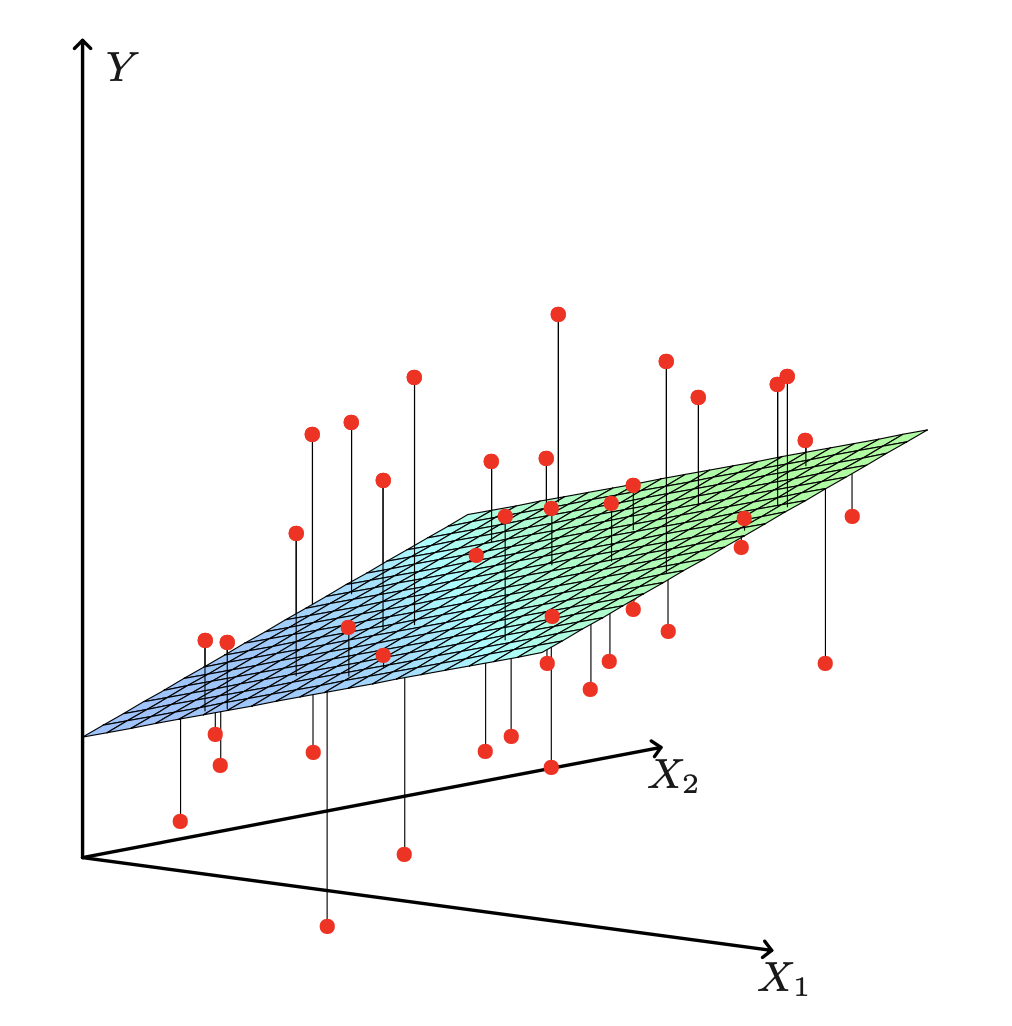
\includegraphics[width=0.39\textwidth]{img/least_squares.png}
\end{figure}
\newpage
How do we minimize Eq. 4.1? Denote by $\boldsymbol{X}$ the $N \times (p + 1)$ matrix with each row an input vector (with a 1 in the first position), and similarly let $\boldsymbol{Y}$ be the $N$-vector of outputs in the training set. Then we can write the residual sum-of-squares as:
\begin{equation*}
    \text{RSS}(\boldsymbol{\theta}) = (\boldsymbol{Y} - \boldsymbol{X\theta})^{\intercal}(\boldsymbol{Y} - \boldsymbol{X\theta})
\end{equation*}
This is a quadratic function in the $p + 1$ parameters. Differentiating with respect to $\boldsymbol{\theta}$ we obtain:
\begin{equation*}
    \pderiv{\text{RSS}}{\theta} = -2\boldsymbol{X}^{\intercal}(\boldsymbol{Y} - \boldsymbol{X\theta})
\end{equation*}
\begin{equation*}
    \frac{\partial^2\text{RSS}}{\partial\theta \partial \theta^{\intercal}} = 2\boldsymbol{X}^{\intercal}\boldsymbol{X}
\end{equation*}
Assuming (for the moment) that $\boldsymbol{X}$ has full column rank, and hence $\boldsymbol{X}^{\intercal}\boldsymbol{X}$ is positive definite, we set the first derivative to zero:
\begin{equation}
    \boldsymbol{X}^{\intercal}(\boldsymbol{Y} - \boldsymbol{X\theta}) = 0
\end{equation}
To obtain the unique solution:
\begin{equation*}
    \hat{\boldsymbol{\theta}} = (\boldsymbol{X}^{\intercal}\boldsymbol{X})^{-1}\boldsymbol{X}^{\intercal}\boldsymbol{Y}
\end{equation*}
The fitted values at the training inputs are:
\begin{equation*}
    \hat{\boldsymbol{Y}} = \boldsymbol{X}\hat{\boldsymbol{\theta}} = \boldsymbol{X}(\boldsymbol{X}^{\intercal}\boldsymbol{X})^{-1}\boldsymbol{X}^{\intercal}\boldsymbol{Y}
\end{equation*}

\begin{figure}[ht]
\caption{The $N$-dimensional geometry of least squares regression with two predictors. The outcome vector $\boldsymbol{Y}$ is orthogonally projected onto the hyperplane spanned by the input vectors $\boldsymbol{x_1}$ and $\boldsymbol{x_2}$. The projection $\hat{\boldsymbol{Y}}$ represents the vector of the least squares predictions.}
\centering
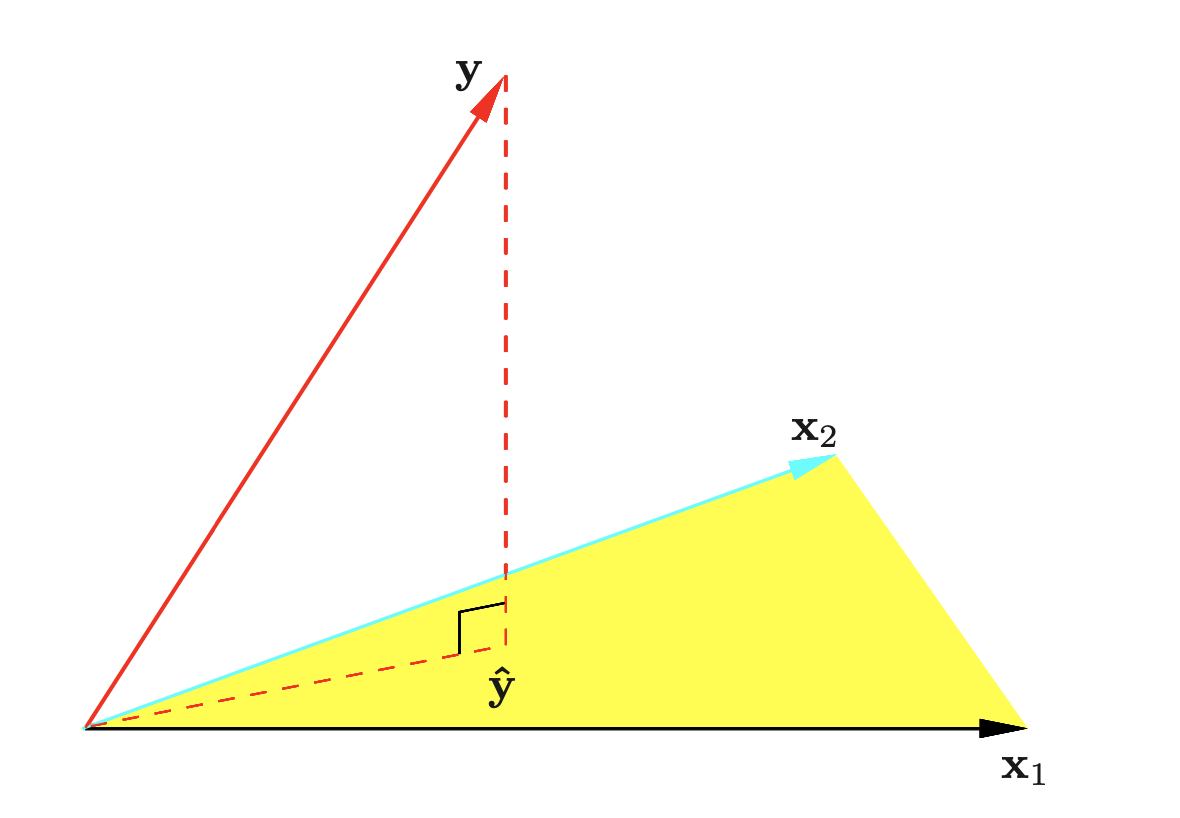
\includegraphics[width=0.39\textwidth]{img/geo_ls.png}
\end{figure}
\newpage
The matrix $\boldsymbol{H} = \boldsymbol{X}(\boldsymbol{X}^{\intercal}\boldsymbol{X})^{-1}\boldsymbol{X}^{\intercal}$ is sometimes called the "hat" matrix because it puts the hat on $\boldsymbol{Y}$.
Figure 4.2 shows a different geometrical representation of the least squares estimate, this time in $\mathbb{R}^N$.
We denote the column vectors of $\boldsymbol{X}$ by $x_0, x_1, . . . , x_p$ with $x_0 = 1$. For much of what follows, this first column is treated like any other. These vectors span a subspace of $\mathbb{R}^N$ , also referred to as the column space of $\boldsymbol{X}$. We minimize $\text{RSS} =  \norm{\boldsymbol{Y} - \boldsymbol{X\theta}}^2$ by choosing $\boldsymbol{\theta}$ so that the residual vector $\boldsymbol{Y} - \boldsymbol{\hat{Y}}$ is orthogonal to this subspace. This orthogonality is expressed in Eq. 4.2, and the resulting estimate $\boldsymbol{\hat{Y}}$ is hence the orthogonal projection of  $\boldsymbol{Y}$ onto this subspace. The hat matrix $\boldsymbol{H}$ computes the orthogonal projection, and hence it is also known as a projection matrix.
\subsection{The Gauss Markov Theorem}
The least squares estimates of the parameters $\boldsymbol{\theta}$ have the smallest variance among all linear unbiased estimates. We will make this precise here, and also make clear that the restriction to unbiased estimates is not necessarily a wise one. This observation will lead us to consider biased estimates such as ridge regression later. We focus on estimation of any linear combination of the parameters $\beta = a^\intercal\theta$; for example, predictions $f(x_0) = x_0^\intercal\theta$ are of this form. The least squares estimate of $a^\intercal\theta$ is:
\begin{equation*}
    \beta = a^\intercal\hat{\theta} = a^\intercal(\boldsymbol{X}^\intercal\boldsymbol{X})^{-1}\boldsymbol{X}^\intercal\boldsymbol{Y}
\end{equation*}
Considering $\boldsymbol{X}$ to be fixed, this is a linear function $c^\intercal\boldsymbol{Y}$ of the response vector $\boldsymbol{Y}$. If we assume that the linear model is correct, $a^\intercal{\theta}$ is unbiased since:
\begin{equation*}
\begin{aligned}
    \mathbb{E}[a^\intercal{\theta}] &= \mathbb{E}[a^\intercal(\boldsymbol{X}^\intercal\boldsymbol{X})^{-1}\boldsymbol{X}^\intercal\boldsymbol{Y}]\\
    &= a^\intercal(\boldsymbol{X}^\intercal\boldsymbol{X})^{-1}\boldsymbol{X}^\intercal(\mathbb{E}[\boldsymbol{X}\theta + \epsilon])\\
    &= a^\intercal(\boldsymbol{X}^\intercal\boldsymbol{X})^{-1}\boldsymbol{X}^\intercal(\boldsymbol{X}\theta + \cancelto{0}{\mathbb{E}[\epsilon]})\\
    &= a^\intercal(\boldsymbol{X}^\intercal\boldsymbol{X})^{-1}\boldsymbol{X}^\intercal\boldsymbol{X}\theta\\
    &= a^\intercal\theta
\end{aligned}
\end{equation*}
\begin{equation*}
\begin{aligned}
    \text{Var}[a^\intercal{\theta}] &= \text{Var}[a^\intercal(\boldsymbol{X}^\intercal\boldsymbol{X})^{-1}\boldsymbol{X}^\intercal(\boldsymbol{X}\theta + \epsilon)]\\
    &= \text{Var}[a^\intercal(\boldsymbol{X}^\intercal\boldsymbol{X})^{-1}\boldsymbol{X}^\intercal\epsilon]\\
    &= \mathbb{E}[a^\intercal(\boldsymbol{X}^\intercal\boldsymbol{X})^{-1}\boldsymbol{X}^\intercal\epsilon\epsilon^\intercal\boldsymbol{X}(\boldsymbol{X}^\intercal\boldsymbol{X})^{-1}a]\\
    &= \sigma^2a^\intercal(\boldsymbol{X}^\intercal\boldsymbol{X})^{-1}a
\end{aligned}
\end{equation*}
\textbf{Alternative unbiased linear estimator} $\widetilde{\beta} = a^\intercal c^\intercal\boldsymbol{Y} = a^\intercal\hat{\theta} + a^\intercal\boldsymbol{DY}$, where $c^\intercal = ((\boldsymbol{X}^\intercal\boldsymbol{X})^{-1}\boldsymbol{X}^\intercal + \boldsymbol{D})$:
\begin{equation*}
\begin{aligned}
    \mathbb{E}[a^\intercal c^\intercal\boldsymbol{Y}] &= \mathbb{E}[a^\intercal\hat{\theta}] + \mathbb{E}[a^\intercal\boldsymbol{DY}]\\
    &= a^\intercal\theta + \mathbb{E}[a^\intercal(\boldsymbol{X\theta} + \epsilon)]\\
    &= a^\intercal\theta + a^\intercal\boldsymbol{DX}\theta + a^\intercal\boldsymbol{D}\cancelto{0}{\mathbb{E}[\epsilon]}\\
    &= a^\intercal\theta
\end{aligned}
\end{equation*}
The unbiasedness condition $\mathbb{E}[a^\intercal c^\intercal\boldsymbol{Y}] = a^\intercal\theta$ implies $\boldsymbol{DX} = 0$.
\begin{theorem}{The Gauss Markov Theorem}\\
For any linear estimator $\widetilde{\beta} = a^\intercal c^\intercal\boldsymbol{Y}$ that is unbiased for $a^\intercal\theta$, that is, $\mathbb{E}[a^\intercal c^\intercal\boldsymbol{Y}] = a^\intercal\theta$, the following holds:
\begin{equation*}
    \text{Var}[a^\intercal\hat{\theta}] \leq \text{Var}[a^\intercal c^\intercal\boldsymbol{Y}]
\end{equation*}
\end{theorem}
\begin{proof}
\begin{equation*}
\begin{aligned}
    \text{Var}[a^\intercal c^\intercal\boldsymbol{Y}] &= a^\intercal c^\intercal \text{Cov}[\boldsymbol{Y}]ca = a^\intercal c^\intercal \sigma^2 \mathds{1} ca = \sigma^2 a^\intercal c^\intercal ca\\
    &= \sigma^2a^\intercal ((\boldsymbol{X}^\intercal\boldsymbol{X})^{-1}\boldsymbol{X}^\intercal + \boldsymbol{D}) (\boldsymbol{X}(\boldsymbol{X}^\intercal\boldsymbol{X})^{-1} + \boldsymbol{D}^\intercal)a\\
    &= \sigma^2a^\intercal((\boldsymbol{X}^\intercal\boldsymbol{X})^{-1}\cancelto{\mathds{1}}{\boldsymbol{X}^\intercal\boldsymbol{X}(\boldsymbol{X}^\intercal\boldsymbol{X})^{-1}} + \boldsymbol{DD^\intercal})a\\
    &= \sigma^2a^\intercal(\boldsymbol{X}^\intercal\boldsymbol{X})^{-1}a + \sigma^2a^\intercal\boldsymbol{DD^\intercal}a\\
    &= \text{Var}[a^\intercal\hat{\theta}] + \underbrace{\sigma^2\norm{\boldsymbol{D}^\intercal a}^2 }_\text{$\geq 0$} \geq \text{Var}[a^\intercal\hat{\theta}]
\end{aligned}
\end{equation*}
\end{proof}

\subsection{The Bias-Variance decomposition}
The use of maximum likelihood, or equivalently least squares, can lead to severe over-fitting if complex models are trained using data sets of limited size. However, limiting the number of basis functions in order to avoid over-fitting has the side effect of limiting the flexibility of the model to capture interesting and important trends in the data. Although the introduction of regularization terms can control over-fitting for models with many parameters, this raises the question of how to determine a suitable value for the regularization coefficient $\lambda$. Seeking the solution that minimizes the regularized error function with respect to both the weight vector $\theta$ and the regularization coefficient $\lambda$ is clearly not the right approach since this leads to the unregularized solution with $\lambda = 0$.\\
The phenomenon of over-fitting is really an unfortunate property of maximum likelihood and does not arise when we marginalize over parameters in a Bayesian setting.\medskip

Each loss function leads to a corresponding optimal prediction once we are given the conditional distribution $p(y | \boldsymbol{x})$. A popular choice is the squared loss function, for which the optimal prediction is given by the conditional expectation, which we denote by $h(\boldsymbol{x})$ and which is given by:
\begin{equation*}
    h(\boldsymbol{x}) = \mathbb{E}[y | \boldsymbol{x}] = \int yp(y | \boldsymbol{x})dy
\end{equation*}
We might use more sophisticated techniques than least squares, for example regularization or a fully Bayesian approach, to determine the conditional distribution $p(y | \boldsymbol{x})$. These can all be combined with the squared loss function for the purpose of making predictions.\\
Armed with the knowledge that the optimal solution is the conditional expectation, we can expand the square term as follows:
\begin{equation*}
\begin{aligned}
    \{\hat{f}(\boldsymbol{x}) - y\}^2 &= \{\hat{f}(\boldsymbol{x}) - \mathbb{E}[y | \boldsymbol{x}] + \mathbb{E}[y | \boldsymbol{x}] - y\}^2\\
    &= \{\hat{f}(\boldsymbol{x}) - \mathbb{E}[y | \boldsymbol{x}]\}^2 + 2\{\hat{f}(\boldsymbol{x}) - \mathbb{E}[y | \boldsymbol{x}]\}\{\mathbb{E}[y | \boldsymbol{x}] - y\} + \{\mathbb{E}[y | \boldsymbol{x}] - y\}^2
\end{aligned}
\end{equation*}
Substituting into the loss function and performing the integral over $y$, we see that the cross-term vanishes and we obtain an expression for the loss function in the form:
\begin{equation}
    \mathbb{E}[L(\boldsymbol{X}, \boldsymbol{Y}; \hat{f})] = \int\{\hat{f}(\boldsymbol{x}) -
    h(\boldsymbol{x})\}^2p(\boldsymbol{x})d\boldsymbol{x} + \underbrace{\int\{ h(\boldsymbol{x}) - y\}^2p(\boldsymbol{x}, y)d\boldsymbol{x}dy}_\text{noise}
\end{equation}
The second term, which is independent of $\hat{f}(\boldsymbol{x})$, arises from the intrinsic noise on the data and represents the minimum achievable value of the expected loss. The first term depends on our choice for the function $\hat{f}(\boldsymbol{x})$, and we will seek a solution for $\hat{f}(\boldsymbol{x})$ which makes this term a minimum. Because it is non-negative, the smallest that we can hope to make this term is zero. If we had an unlimited supply of data (and unlimited computational resources), we could in principle find the regression function $h(\boldsymbol{x})$ to any desired degree of accuracy, and this would represent the optimal choice for $\hat{f}(\boldsymbol{x})$. However, in practice we have a data set containing only a finite number $N$ of data points, and consequently we do not know the regression function $h(\boldsymbol{x})$ exactly.\\
If we model the $h(\boldsymbol{x})$ using a parametric function $\hat{f}(\boldsymbol{x}, \theta)$ governed by a parameter vector $\theta$, then from a Bayesian perspective the uncertainty in our model is expressed through a posterior distribution over $\theta$. A frequentist treatment, however, involves making a point estimate of $\theta$ based on the data set $D$, and tries instead to interpret the uncertainty of this estimate through the following thought experiment:\\
Suppose we had a large number of data sets each of size $N$ and each drawn independently from the distribution $p(x, \boldsymbol{y})$. For any given data set $D$, we can run our learning algorithm and obtain a prediction function $\hat{f}(\boldsymbol{x}; D)$. Different data sets from the ensemble will give different functions and consequently different values of the squared loss. The performance of a particular learning algorithm is then assessed by taking the average over this ensemble of data sets.\medskip

Consider the integrand of the first term in Eq. 4.3, which for a particular data set $D$ takes the form:
\begin{equation*}
    \{\hat{f}(\boldsymbol{x}; D) - h(\boldsymbol{x})\}^2
\end{equation*}
Because this quantity will be dependent on the particular data set $D$, we take its average over the ensemble of data sets. If we add and subtract the quantity $\mathbb{E}_D[\hat{f}(\boldsymbol{x}; D)]$ inside the braces, and then expand, we obtain:
\begin{equation*}
\begin{aligned}
    &\{\hat{f}(\boldsymbol{x}; D) - \mathbb{E}_D[\hat{f}(\boldsymbol{x}; D)] + \mathbb{E}_D[\hat{f}(\boldsymbol{x}; D)] - h(\boldsymbol{x})\}^2\\
    &= \{\hat{f}(\boldsymbol{x}; D) - \mathbb{E}_D[\hat{f}(\boldsymbol{x}; D)]\}^2 + \{\mathbb{E}_D[\hat{f}(\boldsymbol{x}; D)] - h(\boldsymbol{x})\}^2 \\
    &+ 2\{\hat{f}(\boldsymbol{x}; D) - \mathbb{E}_D[\hat{f}(\boldsymbol{x}; D)]\}\{\mathbb{E}_D[\hat{f}(\boldsymbol{x}; D)] - h(\boldsymbol{x})\}
\end{aligned}
\end{equation*}
We now take the expectation of this expression with respect to $D$ and note that the final term will vanish, giving:
\begin{equation*}
\begin{aligned}
    &\mathbb{E}_D[\{\hat{f}(\boldsymbol{x}; D) - h(\boldsymbol{x})\}^2] \\
    &= \underbrace{\{\mathbb{E}_D[\hat{f}(\boldsymbol{x}; D)] - h(\boldsymbol{x})\}^2}_{\text{(bias)}^2}  + \underbrace{\mathbb{E}_D[\{\hat{f}(\boldsymbol{x}; D) - \mathbb{E}_D[\hat{f}(\boldsymbol{x}; D)]\}^2]}_\text{variance}
\end{aligned}
\end{equation*}
We see that the expected squared difference between $\hat{f}(\boldsymbol{x}; D)$ and the regression function $h(\boldsymbol{x})$ can be expressed as the sum of two terms. The first term, called the squared bias, represents the extent to which the average prediction over all data sets differs from the desired regression function. The second term, called the variance, measures the extent to which the solutions for individual data sets vary around their average, and hence this measures the extent to which the function $\hat{f}(\boldsymbol{x}; D)$ is sensitive to the particular choice of data set.\\
So far, we have considered a single input value $\boldsymbol{x}$. If we substitute this expansion back into Eq. 4.3, we obtain the following decomposition of the expected squared loss:
\begin{equation*}
    \textbf{expected loss} = \text{(bias)}^2 + \text{variance} + \text{noise}
\end{equation*}
where:
\begin{equation*}
\begin{aligned}
    &\text{(bias)}^2 = \int \{\mathbb{E}_D[\hat{f}(\boldsymbol{x}; D)] - h(\boldsymbol{x})\}^2 p(\boldsymbol{x})d\boldsymbol{x}\\
    &\text{variance} = \int \mathbb{E}_D[\{\hat{f}(\boldsymbol{x}; D) - \mathbb{E}_D[\hat{f}(\boldsymbol{x}; D)]\}^2] p(\boldsymbol{x})d\boldsymbol{x}\\
    &\text{noise} = \int\{ h(\boldsymbol{x}) - y\}^2p(\boldsymbol{x}, y)d\boldsymbol{x}dy
\end{aligned}
\end{equation*}
and the bias and variance terms now refer to integrated quantities.\medskip

Our goal is to minimize the expected loss, which we have decomposed into the sum of a (squared) bias, a variance, and a constant noise term. As we shall see, there is a trade-off between bias and variance, with very flexible models having low bias and high variance, and relatively rigid models having high bias and low variance. The model with the optimal predictive capability is the one that leads to the best balance between bias and variance.\\
Although the bias-variance decomposition may provide some interesting in- sights into the model complexity issue from a frequentist perspective, it is of lim- ited practical value, because the bias-variance decomposition is based on averages with respect to ensembles of data sets, whereas in practice we have only the single observed data set. If we had a large number of independent training sets of a given size, we would be better off combining them into a single large training set, which of course would reduce the level of over-fitting for a given model complexity.

\section{MLE Regression with Gaussian Noise}
Assumption: noise comes from a zero-mean Gaussian distribution with variance $\sigma^2$, i.e $\epsilon \sim \mathcal{N}(0, \sigma^2)$.\\
Adding a constant to a Gaussian just has the effect of shifting its mean, so the resulting conditional
probability distribution for our generative probabilistic process is:
\begin{equation*}
    \mathbb{P}(\boldsymbol{y_i} | \: \boldsymbol{x_i}, \boldsymbol{\theta}, \sigma^2) = \frac{1}{\sigma\sqrt{2\pi}}\exp{\left \{-\frac{1}{2\sigma^2}(\boldsymbol{y_i} - \boldsymbol{x_i}^{\intercal}\boldsymbol{\theta})\right\}}
\end{equation*}
We denote the noise associated with the $i$th observation as $\epsilon_i$ and we will take these to be independent and identically distributed. This allows us to write the overall likelihood function as a product over these N terms:
\begin{equation*}
    \mathbb{P}(\{\boldsymbol{y_i}\}_{i = 1}^N | \: \{\boldsymbol{x_i}\}_{i = 1}^N, \boldsymbol{\theta}, \sigma^2) = \prod\limits_{i = 1}^N\frac{1}{\sigma\sqrt{2\pi}}\exp{\left \{-\frac{1}{2\sigma^2}(\boldsymbol{y_i} - \boldsymbol{x_i}^{\intercal}\boldsymbol{\theta})\right\}}
\end{equation*}
Now we are going to turn this univariate Gaussian distribution into a multivariate Gaussian distribution with a diagonal covariance matrix:
\begin{equation*}
    \mathbb{P}(\boldsymbol{Y}|\boldsymbol{X},\boldsymbol{\theta}) = \mathcal{N}(\boldsymbol{X}\boldsymbol{\theta}, \sigma^2\mathds{1}) = (2\sigma^2\pi)^{-N / 2}\exp{\left\{ -\frac{1}{2\sigma^2}(\boldsymbol{Y} - \boldsymbol{X\theta})^{\intercal}(\boldsymbol{Y} - \boldsymbol{X\theta}) \right\}}
\end{equation*}
We can now think about how we should maximize this with respect to $\boldsymbol{\theta}$ in order to find the maximum
likelihood estimate. Thus, it is helpful to take the natural log first:
\begin{equation*}
    \log\mathbb{P}(\boldsymbol{Y}|\boldsymbol{X},\boldsymbol{\theta}) = -\frac{N}{2}\log(2\sigma^2\pi) -\frac{1}{2\sigma^2}(\boldsymbol{Y} - \boldsymbol{X\theta})^{\intercal}(\boldsymbol{Y} - \boldsymbol{X\theta})
\end{equation*}
The additive term does not have a $\boldsymbol{\theta}$. We are then left with the following optimization problem:
\begin{equation}
    \boldsymbol{\theta^{\text{MLE}}} = \argmax_{\theta}\left\{ -\frac{1}{2\sigma^2}(\boldsymbol{Y} - \boldsymbol{X\theta})^{\intercal}(\boldsymbol{Y} - \boldsymbol{X\theta}) \right\}
\end{equation}
The $\frac{1}{2\sigma^2}$ does not change the solution to this problem and of course we could change the sign and make
this maximization into a minimization:
\begin{equation*}
    \boldsymbol{\theta^{\text{MLE}}} = \argmin_{\theta}(\boldsymbol{Y} - \boldsymbol{X\theta})^{\intercal}(\boldsymbol{Y} - \boldsymbol{X\theta})
\end{equation*}
This is exactly the same optimization problem for the least-squares linear regression! While it seems like the loss function view and the maximum likelihood view are different, this reveals that they are often the same under the hood: least squares can be interpreted as assuming Gaussian noise, and particular choices of likelihood can be interpreted directly as (usually exponentiated) loss functions.
\subsection{Fitting $\sigma^2$}
One thing that is different about maximum likelihood, however, is that it gives us an additional parameter to play with that helps us reason about the \textit{predictive distribution}. The predictive distribution is the distribution over the label, given parameters we have just fit. Rather than simply producing a single estimate, when we have a probabilistic model we can account for noise when we look at test data.\\
That is, after finding $\boldsymbol{\theta}^{\text{MLE}}$ if we have a query input $\boldsymbol{x_{\text{pred}}}$ for which we do not know the $\boldsymbol{y}$, we could compute a guess via $y_{\text{pred}} = \boldsymbol{x_{\text{pred}}}\boldsymbol{\theta}^{\text{MLE}}$, or we could actually construct a whole distribution:
\begin{equation*}
    \mathbb{P}(y_{\text{pred}}|\:\boldsymbol{x_{\text{pred}}}, \boldsymbol{\theta^{\text{MLE}}}, \sigma^2) = \mathcal{N}(\boldsymbol{x_{\text{pred}}}^{\intercal}\boldsymbol{\theta^{\text{MLE}}}, \sigma^2)
\end{equation*}
We can start by assuming that we have already computed $\boldsymbol{\theta}^{\text{MLE}}$, in order to calculate $\sigma^2$ we set up the problem the same way except we keep the additive term in Eq. 4.4:
\begin{equation*}
    \sigma^{\text{MLE}} = \argmax_{\sigma}\left\{ -\frac{N}{2}\log(2\sigma^2\pi) -\frac{1}{2\sigma^2}(\boldsymbol{X\theta} - \boldsymbol{Y})^{\intercal}(\boldsymbol{X\theta} - \boldsymbol{Y}) \right\}
\end{equation*}
Solving this maximization problem is again just a question of differentiating and setting to zero:
\begin{equation*}
\begin{aligned}
    \pderiv{\left[ -\frac{N}{2}\log(\sigma^2) -\frac{1}{2\sigma^2}(\boldsymbol{X\theta} - \boldsymbol{Y})^{\intercal}(\boldsymbol{X\theta} - \boldsymbol{Y}) \right]}{\sigma^2} &= 0\\
     -\frac{N}{2\sigma^2} + \frac{1}{2\sigma^4}(\boldsymbol{X\theta} - \boldsymbol{Y})^{\intercal}(\boldsymbol{X\theta} - \boldsymbol{Y}) &= 0\\
     -N + \frac{1}{\sigma^2}(\boldsymbol{X\theta} - \boldsymbol{Y})^{\intercal}(\boldsymbol{X\theta} - \boldsymbol{Y}) &= 0 \\
     \sigma^2 = \frac{1}{N}(\boldsymbol{X\theta} - \boldsymbol{Y})^{\intercal}(\boldsymbol{X\theta} - \boldsymbol{Y})
\end{aligned}
\end{equation*}
This is a satisfying result because it is just finding the sample average of the squared deviations between what $\boldsymbol{\theta}^{\text{MLE}}$ predicts and what the training data actually are.

\section{Bayesian Linear Regression}
Bayesian treatment of linear regression avoids over-fitting and also leads to automatic methods of determining model complexity using the training data alone. It makes predictions using all possible parameters, weighted by their posterior probability.\\
Since the likelihood function $\mathbb{P}(\boldsymbol{Y}|\boldsymbol{X},\boldsymbol{\theta}) = \mathcal{N}(\boldsymbol{X}\boldsymbol{\theta}, \sigma^2\mathds{1})$ is the exponential of a quadratic function, the corresponding conjugate prior is defined by $\mathbb{P}(\boldsymbol{\theta}) = \mathcal{N}(0,\Lambda^{-1})$.\\
(N.B Assuming $\Lambda$ and $\sigma^2$ as fixed is a big assumption).\medskip

Now we compute the posterior distribution, which is proportional to the product of the likelihood function and the prior.
\begin{equation*}
\begin{aligned}
    \mathbb{P}(\boldsymbol{\theta}| \boldsymbol{X}, \boldsymbol{Y}) &\propto \mathbb{P}(\boldsymbol{Y}|\boldsymbol{X},\boldsymbol{\theta}) \mathbb{P}(\boldsymbol{\theta})\\
    \log\mathbb{P}(\boldsymbol{\theta}| \boldsymbol{X}, \boldsymbol{Y}) &\propto -\frac{1}{2}\sigma^2(\boldsymbol{Y} - \boldsymbol{X}\boldsymbol{\theta})^\intercal(\boldsymbol{Y} - \boldsymbol{X}\boldsymbol{\theta}) - \frac{1}{2}\boldsymbol{\theta}^\intercal\Lambda\boldsymbol{\theta} + const\\
    &\propto -\frac{1}{2}\boldsymbol{\theta}^\intercal(\sigma^2\boldsymbol{X}^\intercal\boldsymbol{X} + \Lambda)\boldsymbol{\theta} + \boldsymbol{\theta}^\intercal(\sigma^2\boldsymbol{X}^\intercal\boldsymbol{Y}) + const
\end{aligned}
\end{equation*}
By completing the square we note that:
\begin{equation*}
    \Sigma_{\theta} = \sigma^{2}(\boldsymbol{X}^{\intercal}\boldsymbol{X} + \sigma^{2}\Lambda)^{-1}
\end{equation*}
\begin{equation*}
    \mu_{\theta} = \sigma^{-2}\Sigma_{\theta}\boldsymbol{X}^{\intercal}\boldsymbol{y} = (\boldsymbol{X}^{\intercal}\boldsymbol{X} + \sigma^{2}\Lambda)^{-1}\boldsymbol{X}^{\intercal}\boldsymbol{Y}
\end{equation*}
If we consider an infinitely broad prior $\Lambda = \alpha\mathds{1}$ with $\alpha \to 0$, the mean $\mu_\theta$ of the posterior distribution reduces to the maximum likelihood value.\\
Similarly if $N = 0$, then the posterior distribution refers to the prior.\\
Furthermore, if data points arrive sequentially, then the posterior distribution at any stage acts as the prior distribution for the subsequent data point.\\
If we consider a zero-mean isotropic Gaussian governed by a precision parameter $\alpha$ so that:
\begin{equation*}
    \mathbb{P}(\boldsymbol{\theta}|\:\alpha) = \mathcal{N}(\boldsymbol{\theta}|\:0,\alpha^{-1}\mathds{1})
\end{equation*}
The corresponding posterior distribution over $\boldsymbol{\theta}$ has:
\begin{equation*}
    \mu_\theta = \sigma^{-2}(\alpha\mathds{1} + \sigma^{-2}\boldsymbol{X}^{\intercal}\boldsymbol{X})^{-1}\boldsymbol{X}^{\intercal}\boldsymbol{Y} = (\alpha\sigma^2\mathds{1} + \boldsymbol{X}^{\intercal}\boldsymbol{X})\boldsymbol{X}^{\intercal}\boldsymbol{Y}
\end{equation*}
\begin{equation*}
    \Sigma_\theta^{-1} = \alpha\mathds{1} + \sigma^{-2}\boldsymbol{X}^{\intercal}\boldsymbol{X}
\end{equation*}
The $\log$ of the posterior distribution is given by the sum of the log-likelihood and the $\log$ of the prior, and as a function of $\boldsymbol{\theta}$, takes the form:
\begin{equation*}
    \log\mathbb{P}(\boldsymbol{\theta}|\:\alpha) = -\frac{\sigma^{-2}}{2}\sum\limits_{i = 1}^{N}(\boldsymbol{y_i} - \boldsymbol{\theta}^{\intercal}\boldsymbol{x_i})^2 - \frac{\alpha}{2}\boldsymbol{\theta}^{\intercal}\boldsymbol{\theta} + const
\end{equation*}
Maximization of this posterior distribution with respect to $\boldsymbol{\theta}$ is therefore equivalent to the minimization of the sum-of-squares error function with the addition of a quadratic regularization term ($\lambda = \alpha\sigma^2$).
\end{document}